\documentclass[a4paper, 11pt, oneside]{report}
\author{Kyle McMillan kcm40}
\title{TMR IB Project} 
\pagenumbering{roman}


\usepackage[a4paper,left=2.2cm,right=2cm,top=2.5cm,bottom=1.5cm]{geometry}
\usepackage{amsmath}

\usepackage[utf8]{inputenc} % Required for inputting international characters
\usepackage[T1]{fontenc} % Output font encoding for international characters
\usepackage{fouriernc} % Use the New Century Schoolbook font
\usepackage{fancyhdr}
\usepackage{graphicx}
\usepackage{float}
\usepackage{multirow}
\usepackage{hyperref}
\usepackage{verbatimbox}
\setlength{\headheight}{14.49998pt}
\addtolength{\topmargin}{-20.49998pt}

\pagestyle{fancy}
\fancyhf{}% Clear header/footer
\fancyhead[L]{TMR}
\fancyhead[R]{Kyle McMillan, Kcm40}
\fancyfoot[C]{\thepage}% \fancyfoot[R]{\thepage}
\renewcommand{\headrulewidth}{0.4pt}% Default \headrulewidth is 0.4pt
\renewcommand{\footrulewidth}{0.4pt}
% custom commands

\newcommand{\centreImage}[2]{
	\begin{figure}[H]
		\centering
		\includegraphics[width=0.5\textwidth]{#1}
		\caption{#2}
        \label{fig:#1}
	\end{figure}
}
\newcommand{\centreImageTwo}[3]{
    \begin{figure}[H]
        \centering
        \includegraphics[width=0.42\textwidth]{#1}
        \includegraphics[width=0.42\textwidth]{#2}
        \caption{#3}
        \label{fig:#1}
    \end{figure}
}

\newcommand{\centreImageThree}[4]{
    \begin{figure}[H]
        \centering
        \includegraphics[width=0.32\textwidth]{#1}
        \includegraphics[width=0.32\textwidth]{#2}
        \includegraphics[width=0.32\textwidth]{#3}
        \caption{#4}
        \label{fig:#1}
    \end{figure}
}

\usepackage{etoolbox}
\patchcmd{\thebibliography}{\chapter*}{\section*}{}{}
\usepackage{notoccite}

\usepackage{sectsty}

\newcommand{\sdot}{\, {\scriptscriptstyle \odot}\, }
\newcommand\numberthis{\addtocounter{equation}{1}\tag{\theequation}}


\fancypagestyle{firstpage}{
    \fancyhf{}
    \fancyfoot[C]{\thepage}
    \renewcommand{\headrulewidth}{0pt}
}

\fancypagestyle{lastpage}{
    \fancyhead[L]{TMR}
    \fancyhead[R]{Kyle McMillan, Kcm40}
    \fancyfoot[C]{\thepage}% \fancyfoot[R]{\thepage}
    \renewcommand{\headrulewidth}{0.4pt}% Default \headrulewidth is 0.4pt
    \renewcommand{\footrulewidth}{0.4pt}
}

\usepackage[
    backend=biber,
    style=numeric,
    doi=false,isbn=false,url=false,eprint=false,
    sorting=none
]{biblatex}

\addbibresource{CBNN_tmr.bib}


\begin{document}
%----------------------------------------------------------------------------------------
%	TITLE PAGE
%----------------------------------------------------------------------------------------
\thispagestyle{firstpage}
\begingroup
\centering % Centre everything on the title page

{\scshape % Use small caps for all text on the title page

%------------------------------------------------
%	Title
%------------------------------------------------

\rule{\textwidth}{1.6pt}\vspace*{-\baselineskip}\vspace*{2pt} % Thick horizontal rule
\rule{\textwidth}{0.4pt} % Thin horizontal rule

\vspace{0.75\baselineskip} % Whitespace above the title

{\LARGE Efficient Learning In Biological Neural Networks} % Title

\vspace{0.75\baselineskip} % Whitespace after the title block

%------------------------------------------------
%	Subtitle
%------------------------------------------------

Part IB - Technical Milestone Report % Subtitle or further description

\vspace*{1\baselineskip} % Whitespace under the subtitle

%------------------------------------------------
%	Editor(s)
%------------------------------------------------

Edited By

\vspace{0.5\baselineskip} % Whitespace before the editors

{\scshape\Large Kyle McMillan} % Editor list

\vspace{0.5\baselineskip} % Whitespace below the editor list

\textsc{Supervisor: Dr Yashar Ahmadian} % Editor list

\vspace{0.5\baselineskip} % Whitespace below the editor list

\textsc{University Of Cambridge} % Editor affiliation

\vspace{0.75\baselineskip} % Whitespace below the title

\rule{\textwidth}{0.4pt}\vspace*{-\baselineskip}\vspace{3.2pt} % Thin horizontal rule
\rule{\textwidth}{1.6pt} % Thick horizontal rule
}
%----------------------------------------------------------------------------------------
\section*{Abstract}
Artificial neural networks (ANNs) use simple synapses where weights 
are composed of only a single scalar value. However neural synapses contain contain many chemicals that act with a range of dynamic timescales.
This range of timescales is believed to be important for increasing memory capacity and learning efficiency.
This project aims to investigate the impact of using synapses composed of a mixture of dynamical states with a mixture of rigid and plastic
components. To test this we propose a biological update rule called a
recurrent chemical network (RCN) that contains a range of timescales. In order to 
keep with biological plausibility synapses in this network are only updated using local
information. This report presents work undertaken so far and results that show case
an improvement over an earlier model.
\endgroup

\section*{Introduction}

Many systems that are designed to model the brain use traditional artificial neural networks (ANNs) composed of weights made up of scalar values.
However unlike in ANNs, the strength of synapses in the brain are controlled by a range of chemicals that act on a range of timescales.
This abstraction of synapses to a single scalar value is believed to be a limiting factor in the memory capacity and learning efficiency of ANNs.

This project aims to create neural networks where synapses more closely resemble those found in the brain.
Specifically we incorporate a mixture of rigid and plastic components called chemicals
in place of the singular scalar value of ANNs.

\section*{Background}

Biological synapses are composed of many chemicals \cite{1101675601} that alter 
neural plasticity at different timescales.
Phosphorylation of AMPA receptors has been shown to be a rapid short term mechanism 
that affect synaptic plasticity \cite{wang2005}
on the other hand endocannabinoids can act over longer timescales to cause
long term synaptic depression \cite{chevaleyre2007}.

Theoretical models have shown that this range of timescales is important for increasing memory
capacity. Work on simple synapses shows that when bounded the number of memories
grows at best linearly with the square root of then number of synapses \cite{fusi2007}.
However more recent work has shown that complex synapses with plastic and 
rigid components can store memories almost linearly with the number of neurons \cite{benna2016}.
By using a decay mechanism where successive components decay at different rates
in accordance with $\tau^{-k}$ where $k$ is the number of the component and $\tau$ is the time constant, 
the number of memories that can be stored greatly increases.

\subsection*{Learning in Biological Neural Networks}

Traditional ANNs are typically trained using backpropagation:
\begin{equation}
    \Delta w_{ij} = -\eta \frac{\partial E}{\partial w_{ij}}
\end{equation}
where $w_{ij}$ is the weight between neuron $i$ and $j$, $\eta$ is the learning rate and $E$ is the error function.
Backpropagation effectively solves the credit assignment problem (how responsible each weight is 
for the error of the network) by using the chain rule to propagate
errors backwards through the network.
However backpropagation biological implausibility is well documented \cite{lv2024} as it 
requires symmetric weights during it's forward and backwards pass. 
To combat this and explain learning in the brain a number of alternative learning rules have been proposed.

As \cite{richards2019} points out these rules typically follow the path of the gradient, however with a variance and bias.
Some like simulated annealing \cite{szu1987} have an extremely high variance
while others like feedback alignment (FA) \cite{lillicrap2016a} have a high bias. Feedback
alignment is a learning rule where errors are propagated backwards through a network
using fixed random matrices that cause weights to align themselves in this direction.

Specifically we will focus on a biological learning rule proposed by Shervani-tabar in \cite{shervani-tabar2023}.
Shervani-tabar proposes an improvement on FA, where they meta-learn a biological learning rule composed of a set of 10 biological
plausible motifs to update weights of a neural network. These motifs are 
created from combining the activation before and after the weight, the FA error 
before and after the weight and the weight itself. Specifically they focus on 3 specific
motifs as being responsible for the majority of the learning:
\begin{align}
    F^0 &= e_{l}y^T_{l-1} \label{eq2} \\
    F^1 &= e_{l}e^T_{l-1} \label{eq3} \\
    F^2 &= y_{l}y^T_{l-1} - (y_{l}y^T_{l})W_{l-1,l} \label{eq4}
\end{align}

Where $e_{l}$ is the FA error at layer $l$, $y_{l}$ is the activation at layer $l$ and $W_{l-1,l}$ is the weight matrix between layers $l-1$ and $l$.
\ref{eq2} is the FA gradient, \ref{eq3} is a hebbian style error rule that reduces alignment angels between 
weights and a backpropagated basis and \ref{eq4} is Oja's rule.

Weights are then updated using a linear combination of these rules:
\begin{equation}
    W[t+1] = W[t] + \mathbf{P}^T\mathbf{F}
\end{equation}
where $\mathbf{P}$ is the weighting vector that gets meta-learned and $\mathbf{F}$ is the biological motifs.

These adjustments allow the rules to more closely approximate the true gradient
while still being biologically plausible and perform better when compared to pure FA.
However these rules are still limited by the fact the weights are simple synapses.
We aim to extend these rules to work with more complex synapses and will compare to Shervani-Tabar as a baseline.

\subsection*{Meta-Learning}

Meta-learning \cite{schmidhuber1987srl} or learning to learning is the process of optimizing a learning algorithm.
Specifically most meta-learning algorithms involves 2 loops. The inner loop is the learning loop where the model is updated
by a learning rule (in our case the biological learning rule of the RCN) and the outer loop is the meta-learning loop where the learning rule's
meta-parameters are updated. This is typically done calculating the gradient of the loss with respect to the meta-parameters. 

\section*{Methods}

\subsection*{Model and Task}

We implement a 5 layer feedforward neural network with 784-170-130-100-70-47 dimensions where weights are recurrent chemical networks (RCNs).
The network is trained on the EMNIST dataset \cite{cohen2017}.
In order to compare to the Shervani-tabar baseline we implement the same meta-learning algorithm.
Specifically this algorithm involves selecting 5 random classes from the dataset and updating the weights from 50
examples using online learning and the biological learning rule. 10 test examples are then used to calculate the accuracy of the model
and the meta-parameters are updated using the gradient of the loss with respect to the meta-parameters.

\subsection*{Recurrent Chemical Networks (RCNs)}

In order to implement the RCNs we use the following equations:
\begin{align}
    \mathbf{h}[t+1] &= \mathbf{y} \sdot \mathbf{h}[t] + \mathbf{z} \sdot f(K\mathbf{h}[t] + P\mathbf{F}[t] + \mathbf{b}) \label{eq5} \\
    w[t+1] &= \mathbf{v} \cdot \mathbf{h}[t] \label{eq6}
\end{align}
Where $\mathbf{h}$ is the chemical weights, $w$ is the synapse weight, $\mathbf{y}$ is the decay rate, $\mathbf{z}$ is the gain, $\mathbf{F}$ is the Shervani-Tabar biological motifs, $K$ is the recurrent weight matrix, $P$ is the motif weight matrix, $b$ is the bias, $v$ is the weighting of the chemicals
and $f$ is the tanh activation function.
They have sizes: $\mathbf{h} - (L, W), \, \mathbf{y} - L, \, \mathbf{z} - L, \, K - (L, L), \, P - (L, \text{Number of motifs}), \, \mathbf{v} -  L, \, \mathbf{b} - L$.
Where $L$ is the number of chemicals and $W$ is the size of the weight matrix - implementation details mean this can 
either be the actual 2D weight matrix or a flattened 1D weight matrix, both are equivalent.
Meta Parameters $P$, $K$, $v$ and $b$ are meta-learned while $y$, $z$ are fixed, all parameters and the number of chemicals are shared across all layers.
$f$ is the tanh activation function as experimenting has shown it outperforms other activation functions.
$\mathbf{h}$ is randomly initialized to the same values using the Xavier initialization,
$\mathbf{v}$ is initialized as $1/L$ and $K$ and $b$ are initialized to 0. Note the bias is layer specific.

In order to get the range of timescales $\mathbf{z}$ and $\mathbf{y}$ are initialized as follows:
\begin{alignat*}{2}
    \tau_i &= \left( {\frac{\tau_{\max}}{\tau_{\min}}} \right)^{i/L}, \, \, \, &z_i &= \frac{1}{\tau_{min}\tau_i} \numberthis\\
    (y_i)_{i \ne 0} &= 1 - z_i, &y_0 &= 1 \numberthis
\end{alignat*}
Where $\tau_{\max}$ and $\tau_{\min}$ are the maximum and minimum timescales respectively.
We set $\tau_{\max} = 50$ (number of training images) and $\tau_{\min} = 1$.

These equations are a simplified version of the Gated Recurrent Unit (GRU) \cite{cho2014} where the reset gate is removed 
and the update gate is just a non-trainable bias.


\section*{Results}

\subsection*{Baseline Comparison}

\centreImage{individual_3_error.png}{Comparison of the accuracy of the Shervani-Tabar baseline (purple), normal RCN (red) and Layer Dependent RCN (blue).}

Fig\ref{fig:individual_3_error.png} shows the accuracy of the Shervani-Tabar baseline and the RCN model in red with different amount of chemicals per layer.
We find our model outperforms the Shervani-Tabar baseline. However we also find
that the number of chemicals has a fairly negligible impact on the performance of the model as performance of the model
is fairly consistent across the number of chemicals.
Our initial hypothesis would
dictate that the model would perform better with more chemicals and so a larger range of timescales and while there is likely to be a saturation point
this would probably not be reached with the number of chemicals we have used.

\subsection*{Per Layer Learning Rules}

In the previous section the RCN equation \ref{eq5} was the same for all layers. However we can hypothesis that neurons in different layers would require different learning rules.
To test this we make the $P$, $K$, $v$ meta parameters layer specific.

Fig\ref{fig:individual_3_error.png} shows the accuracy of the Shervani-Tabar baseline, the normal RCN and the Layer Dependent RCN.
We find that the layer specific parameters outperform the shared layer parameters.
Especially for the 2 and 3 chemical RCNs where the layer specific parameters outperform the shared layer parameters by a significant margin.

\centreImageTwo{Layers.png}{layerK.png}{Left: $P$ Matrix for the 2 chemical layer dependent RCN for learning rules $F^0$, $F^1$, $F^2$.
Right: $K$ Matrix for 2 chemical layer dependent RCN. Chemical 1 has fast changing timescales while chemical 2 has slow.}

Fig 2 shows the $P$ matrix for the 2 chemical RCN for learning rules $F^0$, $F^1$, $F^2$ - the 3 
most important learning rules highlighted by Shervani Tabar. In the individual layer model case it is extremely interesting specifically
with note to $F^0$. $F^0$ is the pseudo-gradient of the FA error and the activation before the weight. In the shared layer model
this always trains positive - however in the individual layer model it trains negative for some layers and positive for others and seems to alternate.
This could be causing the improvement in performance as it may somehow minimize bias in the propagated errors from the fixed FA weights.

Another very interesting point is that the strength of the $P$ matrix in layer 5 is much larger than the other layers.
This could be optimal however it could also be the result of the meta-learning backpropagation algorithm. Since 
there is no residual connections between layers we could be experiencing a vanishing gradient problem. Further 
investigation is needed to determine if this is the case.

The $K$ matrix for the 2 chemical layer dependent RCN is also shown in Fig 2. It is less interesting than the $P$ matrix however it is worth noting that
the last layer is very different from the other layers. This could be due to the fact that the last layer is the output layer and so the weights need
to be updated differently to the other layers.

\subsection*{Per Neuron Biases}

\centreImageTwo{bias_2.png}{bias_loss.png}{Left: Meta-Accuracy of a RCN with neuron specific biases. Right: Loss of a RCN with neuron specific biases.}

It is extremely unlikely that individual neurons in a layer would have different learning rules -
it would require a degree of complexity that is not biologically plausible. However it is possible that
neurons in a layer could have different biases. To test this we make the $b$ parameter neuron specific.
This makes the bias to have a size of $(L,W)$ where $W$ is the weight matrix size.

Fig 3 present the meta-accuracy and loss of a RCN with neuron specific biases.
These models perform significantly better than all models tested so far. The loss curve shows that 
the model is able to more accurately fit the data and the meta-accuracy curve is much improved.

However there is a chance the model is overfitting. The model could have learnt a specific bias 
for each neuron that is optimal for the training data but not generalizable. To test this we
train the model with only neuron specific biases and no other update motifs. This model doesn't
train at all - it is unable to learn the data. This suggests that the model is not overfitting
the data in this way.

However a disadvantage is that this greatly increases the number of meta-parameters. The number of mta-parameters
in the original RCN was $L^2 + L(\text{Number of update motifs}) + L + Ll$ - where $L$ is the number of chemicals, $l$ is the number of layers.
This corresponds to the number of chemicals squared ($K$), the number of chemicals times the number of update motifs ($P$) and the number of chemicals ($v$) and the number of chemicals times the number of layer ($b$).
The number of meta-parameters in the neuron specific bias model is $L^2 + L(\text{Number of update motifs}) + L + 2LWl$.
This is a huge increase in the number of parameters and could be explain the increase in performance - more parameters
= more capacity to learn the data - however whether or not this is biologically plausible is another question.

Further work is needed to determine if this is the case. Specifically the bias needs to be further investigated to see 
how it is acting (if it is acting as some sort of edge highlighter in early layers for example this is much more biological plausible).
Secondly this trained RCN needs to be tested on another dataset to see if it is generalizable.

\subsection*{Adjusting the RCN Output}

\begin{figure}[H]
    \centering
    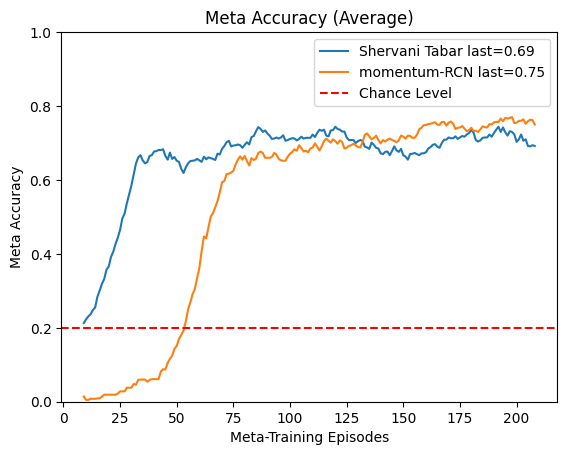
\includegraphics[width=0.4\textwidth]{mode3.png}
    \caption{Meta accuracy of a 5 chemical RCN with momentum output}
    \label{fig:mode3}
\end{figure}

The RCN output is currently a linear combination of the chemical weights as defined in equation \ref{eq6}.
However an alternative RCN called the momentum-RCN could be constructed where the output rule is instead:
\begin{equation}
    w[t+1] = \mathbf{v} \cdot \mathbf{h}[t] + w[t]
\end{equation}

A particularly interesting point here is
that when expressed in this way the RCN would be approximately equivalent to a gradient descent
with momentum. This provides a biological plausible explanation for the momentum term in gradient descent.


Fig\ref{fig:mode3} shows the meta-accuracy of a 5 chemical RCN with momentum output. This model slightly outperforms Shervani-Tabar,
however further work would need to be done on the optimal initialization of chemical weights and the optimal number of chemicals
as well as what $y$ and $z$ should be.

\section*{Discussion and Future Work}

Overall the work so far presents an introduction of a biological plausible learning rule in the RCN model.
Results indicate that the model outperforms the Shervani-Tabar baseline and the further modifications
such as layer specific parameters and neuron specific biases improve the model further. However
we also find that the number of chemicals past 1 has a negligible impact on the performance of the model.
Lastly we present a major modifications in the form of the momentum-RCN which could provide a biological
plausible explanation for momentum in the brain.

Future work will go down two paths. The first is an adjustment to the meta-training task.
Classification may not utilize the full potential of chemicals with different timescales so 
migrating to a regression task may be more appropriate. The second is to investigate more architectural 
changes to the RCN. Perhaps the first major change is to make the RCN $y$ and $z$ parameters depend on the chemicals
themselves like in the GRU. This would allow the model to learn the optimal timescales for each chemical and
is biological plausible as chemical timescales like the endocannabinoids are dependent on other chemicals for their
timescales. A second architectural change to be investigated is to make the fixed FA weights adaptable and train
a RCN rule to update them. This would allow the model to learn the optimal feedback weights for the task at hand
and may offer a way to get closer to backpropagation's performance.

%\bibliographystyle{unsrt}
%\bibliography{CBNN.bib}
{
\renewcommand{\clearpage}{} % Prevents a page break at the start of the bibliography
\AtNextBibliography{\small}
\printbibliography
\thispagestyle{lastpage}
}

\end{document}


